\chapter[Artefatos dos Brainstorm]{Artefatos dos Brainstorm} \label{apendices:brainstorms}

\begin{figure}[H]
	\centering
	\includegraphics[keepaspectratio=true,scale=0.3]{figuras/brainstorm/brainstorm1.eps}
	\caption{Brainstorm de definição de Release}
	\label{}
\end{figure}

\begin{figure}[H]
	\centering
	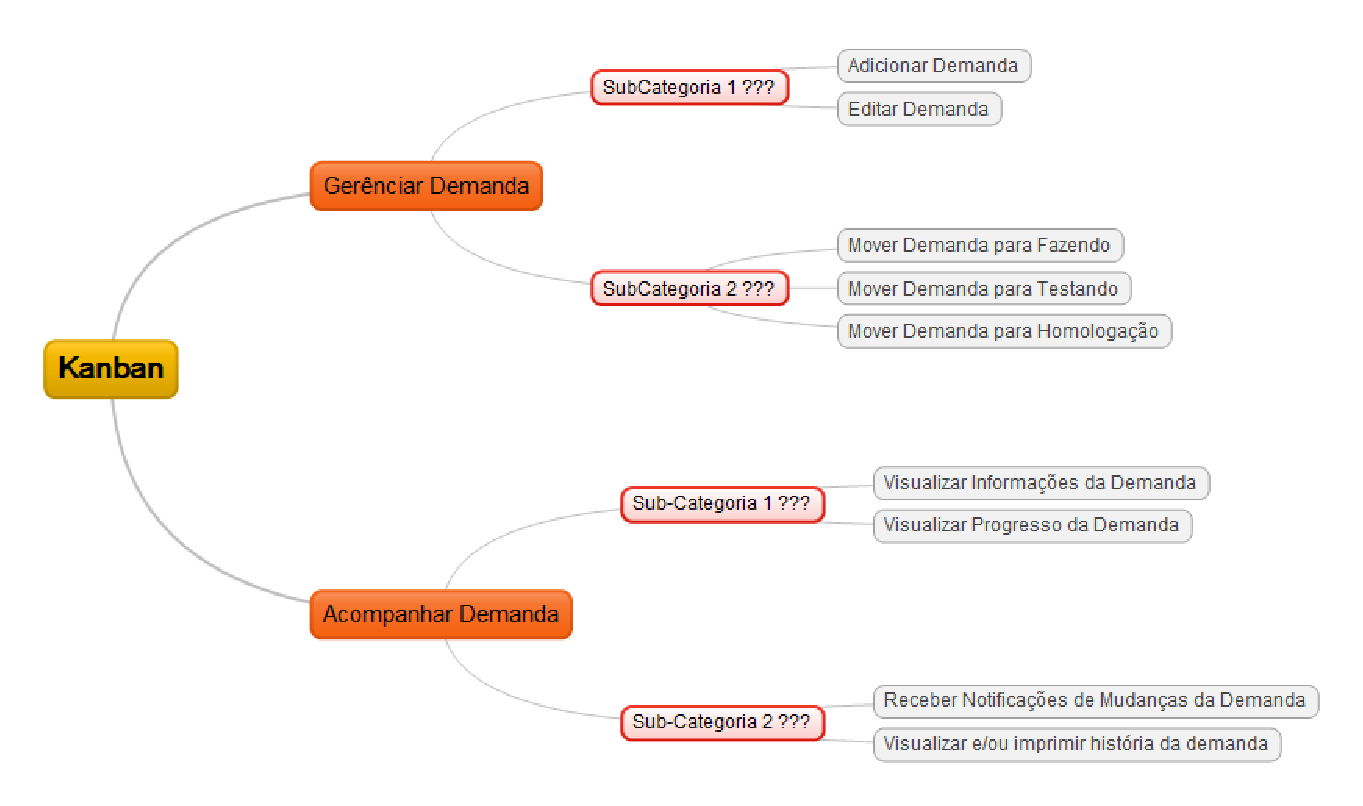
\includegraphics[keepaspectratio=true,scale=0.8]{figuras/brainstorm/brainstorm2.eps}
	\caption{Brainstorm sobre épicos}
	\label{}
\end{figure}

\begin{figure}[H]
	\centering
	\includegraphics[keepaspectratio=true,scale=0.5]{figuras/brainstorm/brainstorm3.eps}
	\caption{Brainstorm sobre funcionalidades}
	\label{}
\end{figure}

\begin{figure}[H]
	\centering
	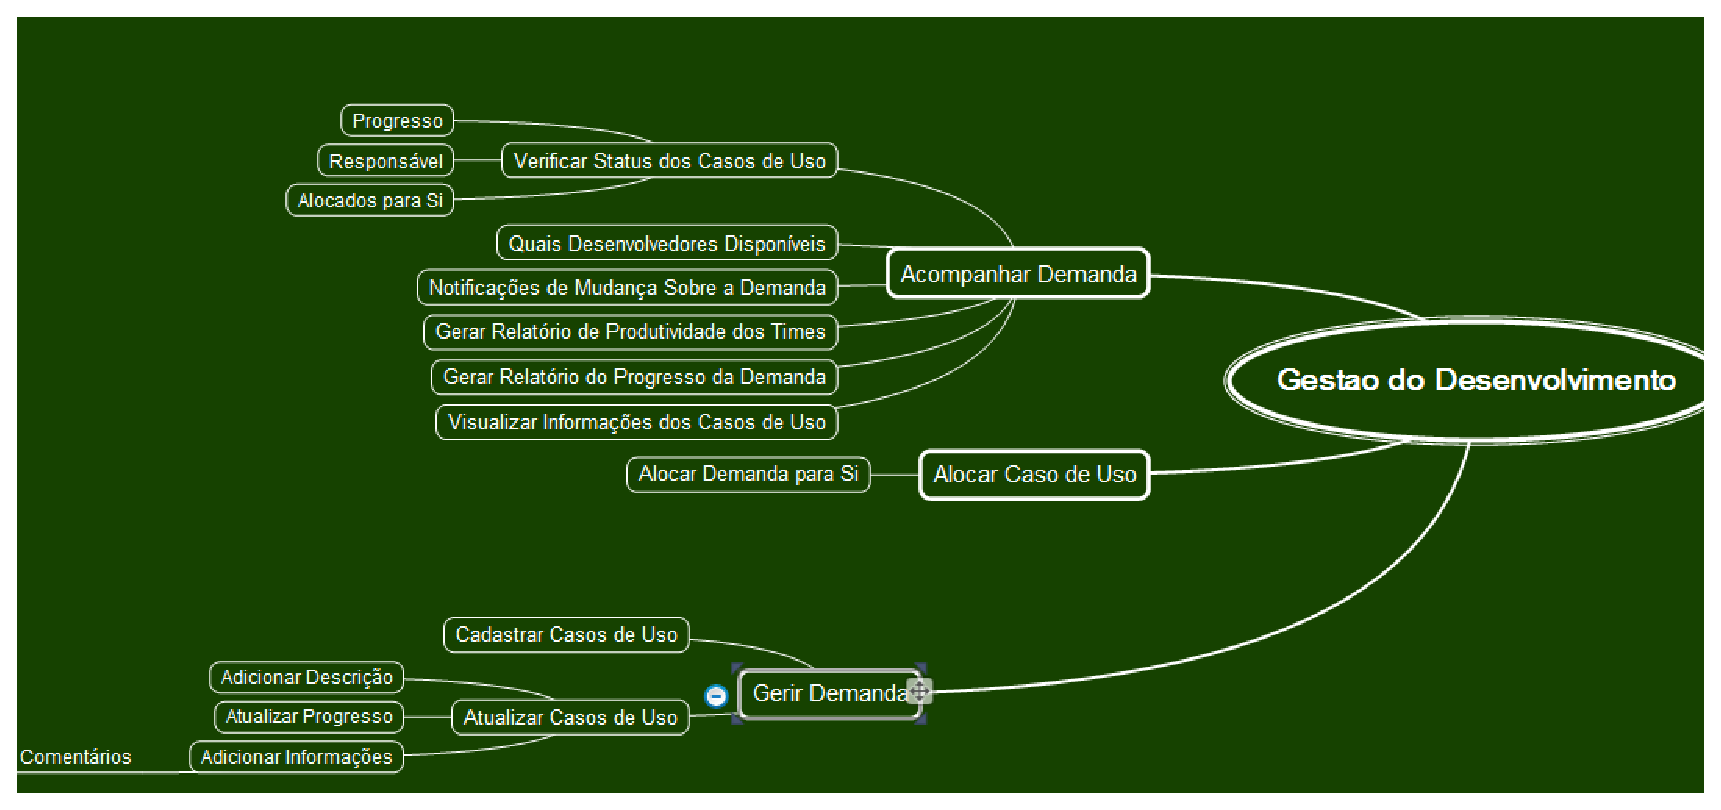
\includegraphics[keepaspectratio=true,scale=0.6]{figuras/brainstorm/brainstorm4.eps}
	\caption{Brainstorm de épicos e features}
	\label{}
\end{figure}

\section{Agenda Workshop do dia 19/10}

Workshop é uma evento, onde todos tem espaço para expor suas idéias, com tempo definido.
Workshop e agenda inspirado e baseado em \cite{UFPRUNI2}

\begin{table}[H]
	\begin{tabular}{|l|l| p{8cm} |}
		\hline 
		Período & Item & Descrição\tabularnewline
		\hline 
		\hline 
		12:00 - 12:10 & Introdução & Revisar agenda e regras\tabularnewline
		\hline 
		12:20 - 12:40 & Contexto & Apresentar o estado do processo, as necessidades, os resultados das
		entrevista com o cliente e demais\tabularnewline
		\hline 
		12:40 - 13:40 & Brainstorm & Aberto para 15 minutos de exposição de idéias\tabularnewline
		\hline 
		13:40 - 14:00 & Definição e Fecho & Revisar principais grandes idéias e guarda-las para o próximo workshop\tabularnewline
		\hline 
	\end{tabular}
\end{table}

\subsection{Relatório do Workshop 1}

Inicialmente ouve uma reunião entre MPR, Req(GP e dois membros) e o cliente de MPR, nessa reunião a equipe de requisitos não se manifestou, apenas observou para facilitar o entendimento do contexto em que MPR está inserido.

Após este evento, foi iniciado o workshop entre MPR e Req(Toda a equipe) com o objetivo de indentificar os temas de investimentos. Para isso, o workshop(Debate Livre) seguiu a seguinte agenda -> Referencia <-, os membros de MPR narraram o processo to be, apontaram os gates onde foram indentificados os maiores problemas e após isso, foi iniciado o debate para melhorar a consistência do entendimento do problema entre ambos, neste debate foi utilizado a tecnica de brainstorm. 

Durante o debate, houve dificuldade para o consenso sobre o problema relacionado a teste de software no processo do cliente, entretanto após um longo debate, chegou-se a conclusão que o grande problema se resumia a comunicação entre as entidades presentes no processo.

A equipe de MPR junto com o cliente durante a primeiro evento, proporam as seguintes soluções:

\begin{itemize}
	\item Formulário para requisição da manutenção do software

	\item Automatização dos testes

	\item Feedback do usuário
\end{itemize}

A partir desse problema e propostas, chegou-se ao consentimento dos seguintes temas de investimentos:

\begin{itemize}
	\item \textbf{Padronização da Comunicação}
		\begin{itemize}
			\item Devido a falta de consistência entre a demanda e o produto entregue, é necessário uma comunicação padronizada para garantir o entendimento entre os envolvidos.
		\end{itemize}
	\item \textbf{Geração Feedback Contínuo}
		\begin{itemize}
			\item Devido ao custos gerado pelo fato de que o cliente obtém e dá feedback apenas no fim do processo.
		\end{itemize}
\end{itemize}


\subsubsection{Questionários}

Após o brainstorm, os resultados foram validados com o professor e devidamente reprovados, gerando a necessidade da criação de um questonário para esclarecimento do escopo do processo do cliente.

\textbf{Na atividade de especificar a demanda:}
\begin{itemize}
	\item Como é feito esta atividade? 
	\item Como é armazenado o documento? 
	\item Como é enviado para outro departamento(Qualidade)?
\end{itemize}

\textbf{Na atividade de Contagem de ponto de funções:}
\begin{itemize}
	\item Como a contagem de ponto de função é enviado para DISIS?
\end{itemize}

\textbf{No Gateway de escolher se a manutenção é evolutiva ou corretiva:}
\begin{itemize}
	\item Como é e feita a decisão se a manutenção é evolutiva ou corretiva? 
	\item Como as informações são recebida? 
	\item Quais informações são necessárias para tomar a decisão?
\end{itemize}

\textbf{Na atividade de evolução de software:}
\begin{itemize}
	\item Como é distribuido a demanda para ser desenvolvida(Evolui Software)?  
	\item Quem distribui a demanda e de qual forma?
	\item Como ele distribui?
	\item Como ele entrega essa demanda para o desenvolvedor?
	\item Como ele Escolhe qual desenvolvedor irá desenvolver a demanda ? 
\end{itemize}

\textbf{Na atividade de teste de software:}
\begin{itemize}
	\item Como o software evoluido é passado para ser testado?  
	\item Quais informações recebe para fazer o teste? 
	\item Quais Informações são passadas para a equipe de qualidade ?
\end{itemize}

\textbf{Publica código para a homologação:}
\begin{itemize}
	\item Como é publicado o código para a homologação ?
	\item Nessa etapa como é a relação entre a equipe de manutenção e o cliente ? 
\end{itemize}

\textbf{A equipe de manutenção sabe se o usuário gestor aprovou ou recusou a solução ?}

\section{Relatório da Reunião Para Correção de Inconsistências do Dia 13/11}

Foi realizado uma reunião entre Requisitos e MPR devido a necessidade de corrigir instabilidades no processo do cliente. Assim, chegou-se nas seguintes definições:

\begin{itemize}
	\item Demanda
		\begin{itemize}
			\item Um desenvolvedor vincula uma demanda por vez no kanban (RN)

			\item Novas demandas entram na fila de espera. (RN)

			\item Demandas urgentes “furam” a fila de espera e se tornam primeras na fila de espera. (RN)

			\item Um desenvolvedor ao está disponível pega a próxima demanda na fila de espera (RN)

			\item Um desenvolvedor após implementar a demanda, a demanda entra em teste pelo próprio desenvolvedor. (RF)

			\item Após o teste a demanda é enviada para homologação (RF)
		\end{itemize}
	\item Gerente de Manutenção
		\begin{itemize}
			\item O gerente de manutenção é responsável por adicionar uma nova demanda no sistema. (RF)

			\item O sistema, no momento em que o gerente adiciona a nova demanda, a partir do email em que foi preenchido ser do cliente, o sistema envia para o email um id onde o cliente poderá acompanhar o progresso da demanda. (RN)
		\end{itemize}
	\item Cliente
		\begin{itemize}
			\item O cliente, a partir de um id enviado para o seu email, acessa o sistema e após informar o id, consegue acompanhar o progresso da demanda. (RF)
			\item Quando a demanda for finalizada e enviada para homologação, o cliente é avisado por email, onde pelo sistema ele poderá homologar a demanda ou recusar. (RN)
		\end{itemize}
\end{itemize}
